\chapter{Distributed Storage Systems}

\section{The CAP Theorem}
	The CAP theorem relates the following three properties:
	\begin{itemize}
		\item \textbf{Consistency}: Every operation must appear to take effect in a single indivisible point in time between its invocation and response.
		\item \textbf{Availability}: Every client's request is served (receives a response) unless a client fails (despite a strict subset of server nodes failing).
		\item \textbf{Partition tolerance}: A system functions properly even if the network is allowed to lose arbitrarily many messages sent from one node to another.
	\end{itemize}
	To sacrifice P implies that the system does not function properly, therefore it sacrifices C or A. In the same way, negating P means that the system is not allowed to lose arbitrarily many messages, but in practice it is not possible to choose whether the network will lose messages or not.\newline
	In practical distributed systems partitions may occur and this is not under the system designer control. The designer choice is between C and A when/if temporary partitions occur.\newline
	In summary, \textbf{practical distributed systems are either CP or AP, the choice depends on the application logic}.

\section{Amazon Dynamo}
	\subsection{Overview}
	Amazon Dynamo is behind the Amazon Web Services. AWS is AP (sacrifices consistency), and follows the BASE philosophy (no ACID): Basically Available, Soft state, \textbf{Eventually consistent}.\newline
	Clearly, consistency violations have significant financial consequences and impact customer trust, but not in several Amazon services (billing is separated).\newline
	\newline
	Dynamo is an highly available key-value storage system that favours availability over consistency under failures.\newline
	It has a simple API (\textit{get(), put()}) that uses and additional argument to pass a \textit{context}, holding critical metadata (typically small).\newline
	Amazon Dynamo main features are:
	\begin{itemize}
		\item Low latency
		\item Scalability
		\item Always-on, available
		\item Partition and fault tolerance
		\item \textbf{Eventually} consistency
	\end{itemize}
	The design is made to have an \textbf{always writable} data store that allows multiple versions of data and \textbf{reconciles and resolves conflicts during reads}. Conflicts are solved depending on the business logic on the application size and in a deterministic way (last write) on the Dynamo side.\newline
	Failure detection is unreliable, the detection is triggered by read/write requests (in band detection), there is no dedicated component. \textbf{It does not make the distinction between faults and partitions}.
	\subsection{Data partitioning and consistent hashing}
	Dynamo uses dynamic partitioning of keys over a set of storage nodes (technique used for DHTs).\newline
	The hashes of keys give m-bit key identifiers and the hashes of nodes give m-bit node identifiers. Identifiers are ordered in a circle.\newline
	A key \textit{k} is assigned to the closest \textbf{successor node}, the first node whose $ID\geq k$. If such node does not exist, navigate the circle and find the node with the smallest \textit{ID}.
		\subsubsection{Dynamic membership management}
		Storage nodes can come and go to allow incremental \textbf{scalability}.\newline
		If node \textit{n} joins then the keys previously assigned to \textit{n}'s successor are now assigned to \textit{n}. If node \textit{n} leaves, all keys currently assigned to him are assigned to its successor.
		\subsubsection{Load balancing}
		Each node is responsible for at most $(1 + \epsilon) K / N$ keys. When a node joins, only $O(k/n)$ keys must be moved (optimal).\newline
		Moreover, each physical storage node is mapped multiple times to the circle (\textbf{virtual nodes}) to improve load balancing and allow heterogeneous storage nodes.
		\subsubsection{Data replication}
		To achieve high \textbf{availability} and \textbf{durability} each key is replicated at \textit{N} nodes (virtual nodes are skipped), where \textit{N} is configurable.\newline
		If \textit{N = 3} and \textit{B} is the \textit{coordinator} for key \textit{k}, then \textit{B} replicates \textit{k} in \textit{N - 1} successor nodes (\textit{C, D}). The ordered list of coordinator and successor nodes (\textit{B, C, D}) is the \textbf{preference list} of \textit{k}.
	\subsection{Data versioning with Vector Clocks}
	Data replication is performed after an ACK is sent to a client \textit{put} request. \textbf{Asynchronous replication} may result in inconsistencies under partitions.\newline
	If an operation is performed when the latest version is not available, then it is performed on a stale version of the data: there could be different versions of a key-value pair.\newline
	Once a partition heals, different versions must be merged, new versions subsume previous ones.\newline
	\newline
	Each write to a key \textit{k} is associated to a vector clock \textit{VC(k)} which is an array of integers. In theory there is one entry \textit{VC(k)[i]} for each storage node \textit{i}, it is incremented when node \textit{i} handles a write for key \textit{k}.\newline
	In practice \textit{VC(k)} has only entries for nodes from the preference list, Dynamo truncates entries if there are more than a threshold.
		\subsubsection{Anatomy of \textit{put} and \textit{get}}
		Storage nodes can receive requests for any key, a load balancer chooses a random node, not necessarily the coordinator.\newline
		If a request comes from the load balancer, the node serves it only if it is in the preference list, otherwise it routes it to the first node in the preference list. All nodes know all other nodes because of \textbf{0-hop DHT routing}, this is not the most scalable technique but it is excellent for low latency.\newline
		An \textbf{extended preference} list accounts for node failures.
	\subsection{Handling failures with quorums}
	The quorum system uses three parameters: \textit{R + W $>$ N}, where \textit{N} is the number of replicas.\newline
	When the coordinator receives a \textit{put} it generates a new \textit{VC} and writes the new version locally, then it send the value to \textit{N} nodes from the preference list and waits for \textit{W - 1} acknowledgements.\newline
	For the \textit{get}, it sends the request to \textit{N} selected nodes from the preference list and waits for \textit{R} responses, then it selects the highest versions using VCs and reconciles/merges them. Finally, it writes back the reconciled version.\newline
	\newline
	\textit{R} and \textit{W} should be smaller than \textit{N} to decrease the latency, that is the time taken by the slowest replica. If \textit{W = 1} the system is always available for writes but it pays back for the reads, \textit{R = N}. Dynamo's typical values are \textit{W, R, N = 2, 2, 3}.\newline
	\newline
	The \textit{N} selected nodes are the first \textit{N} healthy nodes, they may change from request to request (sloppy quorums). Sloppy quorums allow availability under a wider range of partitions and in case of failures, but they sacrifice consistency.\newline
	If a replica in the preference list is down, then the coordinator creates a new replica on a new node, but hints that the role is temporary (\textbf{hinted handoff}). When the new replica learns about failure recovery it handles data to the node in the preference list.
	\subsection{Anti-entropy replica synchronization}
	This mechanism uses \textbf{Merke trees}, every non-leaf node is labelled with the hash of the labels of its children nodes.\newline
	Storage nodes keep a Merkle tree for each of their virtual nodes and compare the root of the tree with replicas, if they're equal, then they're synced, otherwise, traverse the tree and synchronize keys that differ.
	\subsection{Gossip membership management}
	Membership management is initiated by the administrator, the gossip protocol propagates membership changes.\newline
	Nodes contact a random node every second and couples of nodes reconcile membership information.\newline
	Gossip is also used to handle metadata.

\section{Apache HBase}
	\subsection{From RDBMS to NOSQL}
	Column oriented databases save their data grouped by columns, subsequent column values are store contiguously on disk.\newline
	This kind of database is used for specific workloads, they are better suited for compression but they support reduced I/O.\newline
	HBase is not a column-oriented DB in the typical form, it just uses an on-disk column storage format and provides key-based access to specific cells or sequential ranges of data.\newline
	\newline
	The problem of RDBMS is that, even if different solutions can be applied, they are not really good at scaling to big amounts of data.\newline
	Non-relational databases originally do not support SQL (NOSQL), the main differences are in the data model and the consistency model: ACID and transactions are generally sacrificed.\newline
	There are different dimensions to classify NOSQL databases:
	\begin{itemize}
		\item \textbf{Data model}: how data is stored (key-value, semi-structured, column oriented); how to access data and how can the schema evolve.
		\item \textbf{Storage model}
		\item \textbf{Consistency model}
		\item \textbf{Physical model}
		\item \textbf{Read/Write performance}
		\item \textbf{Secondary indexes}
		\item \textbf{Failure handling}
		\item \textbf{Compression}
		\item \textbf{Load balancing}
		\item \textbf{Atomic read-modify-write}
		\item \textbf{Locking and deadlocks}
	\end{itemize}
	It is not possible to have a unique solution, each problem has its own match.\newline
	\newline
	A good methodology to scale the schema design is to apply DDI: Denormalization, Duplication and Intelligent key design. Wide tables and column-oriented design eliminates joins, but compound keys are essential and data partitioning is based on keys therefore a proper understanding of them is needed.
	\subsection{Table, Rows, Columns and Cells}
	The mist basic unit in HBase is a column, each column may have different versions with each distinct value in a separate cell. One or more columns form a row which is uniquely addressed by a row key. All\textbf{ rows are sorted lexicographically} by their row key.\newline
	\newline
	Columns are grouped into \textbf{column families} that are stored together in the same low-level storage file: the HFile. They are defined when the table is created so they should not be changed too often and their number should be reasonable because of metadata.\newline
	Column family name is composed by printable characters. Row key and column name (\textit{qualifier}) can be any arbitrary array of bytes.\newline
	A column is referenced though his \textbf{column key}: family:qualifier.\newline
	\newline
	In RDBMS \textit{null} cells need to be set and occupy space, in HBase they are simply not stored.\newline
	Every column value (cell) is timestamped for versioning. Cell versions can be constrained by predicate deletions (e.g. keep only valued from last week).\newline
	\newline
	Data can be represented as follows: \textit{SortedMap<RowKey, List<SortedMap<Column, List <Value, Timestamp>>>>}, where the first sorted map is the table containing a list of column families and each column family is a list of columns containing a list of value-timestamp tuples.\newline
	\newline
	HBase is strongly consistent, row data access is \textbf{atomic} and includes any number of columns. There is no other feature spanning multiple rows.
	\subsection{Automatic Sharding}
	A \textbf{region} is the basic unit of scalability and load balancing, they are contiguous ranges of rows stored together, they are dynamically split at the middle key when they become too large and they can be merged to reduce the number of storage files.\newline
	Each region is served by exactly one \textbf{region server}. The number of region servers depend on their capability, each region server can serve multiple regions.\newline
	Regions allow fast recovery upon server failures, the HDFS handles the replication automatically.\newline
	Fine-grained load balancing is achieved thanks to region because they can easily be moved across servers.
	\subsection{Storage API}
	There is no support for SQL, CRUD operations are implemented by a standard API.\newline
	The \textbf{Scan API} allows for fast iteration over ranges of rows, limit the number and which column are selected, control the version number of each cell.\newline
	The \textbf{read-modify-write API} allows single row  transactions.\newline
	\newline
	Counters are updated atomically, they are global, strongly consistent and sequential.\newline
	Coprocessors allow to push user code in the server and access server's local data in order to implement lightweight batch jobs, data preprocessing and data summarization.
	\subsection{HBase Implementation}
		\subsubsection{Data Storage}
		Store files are called \textbf{HFiles}, they are persistent and \textbf{ordered immutable maps} from key to value.\newline
		They are internally implemented as sequences of blocks with an index at the end, the index is loaded when the HFile is opened, and then kept in memory.
		\subsubsection{Data lookups}
		Since HFiles have a block index, lookup can be done with a single disk seek. First, the block possibly containing a given lookup key in determined with a \textbf{binary search} in the in-memory index, then a block read is performed to find the actual key.
		\subsubsection{Write operation}
		First, data is written into a commit log (Write-Ahead-Log), then it is moved into memory, in a structure called \textbf{memstore}. When the size of the memstore exceeds a given threshold, it is flushed into an HFile into disk.\newline
		\newline
		In order to handle reads and writes together, HBase uses a \textbf{rolling mechanism}: new and empty slots of the memstore take the updates, while the old and full slots are flushed to disk.\newline
		Data in memstore is sorted by keys as in the HFiles.
		\subsubsection{Data Locality}
		Data locality is achieved through intelligent key design and by the system looking up for server hostnames.
		\subsubsection{Deleting Data}
		HFiles are immutable, therefore in order to delete data a delete marker (tombstone marker) is written to indicate that a given key is deleted.\newline
		During the read process, data marked a sdeleted is skipped and compactions finalize the deletion process.
		\subsubsection{Read operation}
		During the read, data in the memstores (not on disk) and in the HFiles is merged. The WAL is never used in the read operation.
		\subsubsection{Compactions}
		Flushing data from memstores to disk implies the creation of new HFiles each time, therefore we end up with many (probably small) files and we need to do housekeeping.\newline
		In the case of \textbf{minor compaction} it rewrites small HFiles into fewer, larger ones using an n-way merge.\newline
		In the case of \textbf{major compaction} it rewrites all files within a column family or a region in a new one. It drops deleted data and performs predicated deletion (old data).
	\subsection{Architecture}
		\begin{figure}[H]
			\centering
			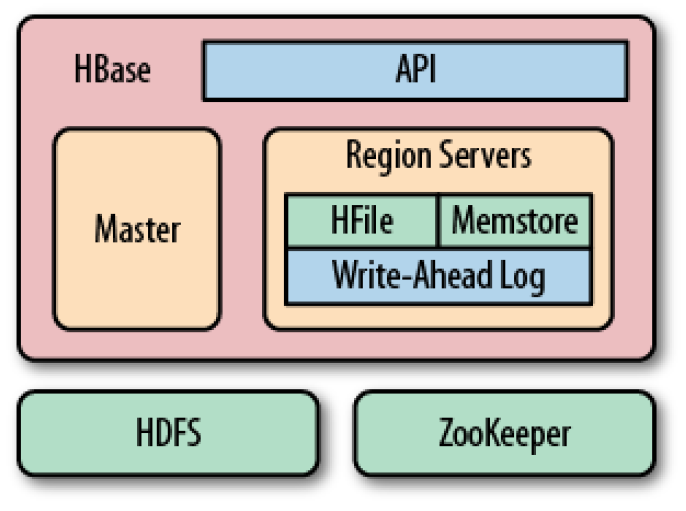
\includegraphics[width=0.5\linewidth]{images/hbasearch.png}
		\end{figure}
		\subsubsection{Overview}
		The master node (HMaster) assigns regions (key space) to region servers using zookeeper, handles load balancing (ZooKeeper) and holds metadata and schema.\newline
		Region servers handle reads and writes, the WAL and HFiles, and region splitting.
		\subsubsection{B+ Trees vs LSM Trees}
		B+ Trees use dynamic, multi-level indexes for efficient insertion, lookup and deletion. Frequent updates may imbalance the tree and a costly re-organization is required.\newline
		They support large scans, no costly tree-traversal algorithm is needed.\newline
		Updated and deletes are done at disk seek rates, rather than transfer rates.\newline
		\newline
		LSM Trees work at disk transfer rate and scale better to huge amounts of data. They guarantee a consistent insert rate (transforming random writes into sequential ones).\newline
		Reads are independent from writes. The optimized data layout offers predictable boundaries on disk seeks.
		\begin{figure}[H]
			\centering
			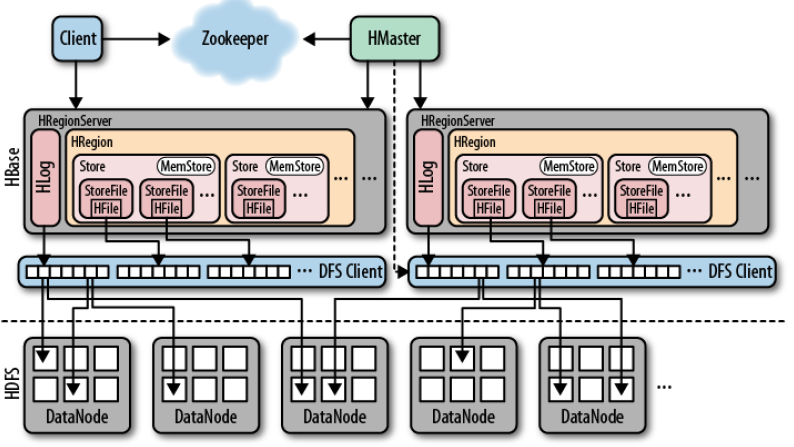
\includegraphics[width=0.7\linewidth]{images/hbasestorage.png}
		\end{figure}
	\subsection{Key Design}
		HBase has two fundamental key structures> row key and column key, they store meaningful data and their sorting is important.
		\subsubsection{Logical and physical layout of a table}
			 The main unit of separation within a table is the column family. Differently than the traditional column-based DBs, columns are not used to separate data, cells are stored logically in a table format and rows are stored as linear sets of cells.\newline
			 In the logical layout the table consist of rows and columns, this layout is folded so that the cells of each row are stored one ofter the other but each column family is stored separately (cells of one family reside on an individual HFile). HBase does not store unset cells.
			 Multiple versions of the same cell are stored consecutively, together with the timestamp, they are ordered in descending order so that the newest value is the first.
			 \begin{figure}[H]
			 	\centering
			 	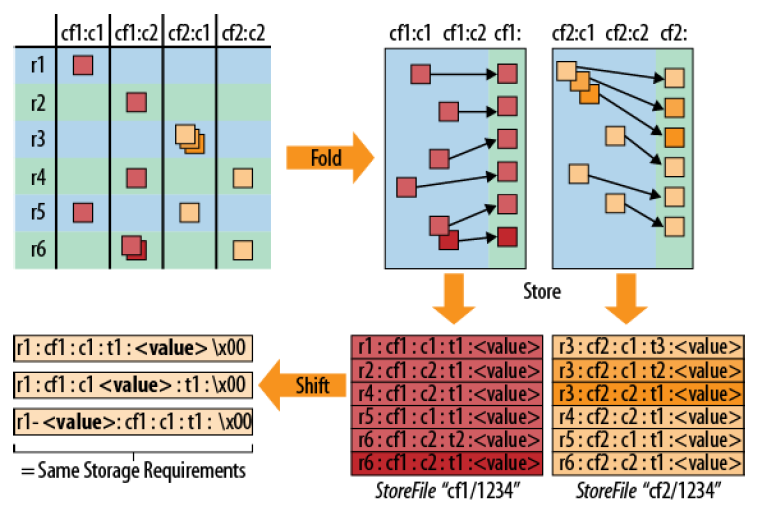
\includegraphics[width=0.65\linewidth]{images/hbaselayout.png}
			 \end{figure}
			 From the physical layout it is possible to select data by row-key from the different StoreFiles, this reduces the amount of data to scan for a row or a range of rows. When selcting data by row and column key, the system focuses on an individual storage. If the column qualifier is used, the system uses exact lookups, including filters to omit useless data.\newline
			 \newline
			 Given this query granularity, it is recommended to have tall-narrow tables with few columns and many rows.\newline
			 When missing the column key, the partial key scan allows to scan all the values for a given row key.
		\subsubsection{Time Series Data}
			If we use the timestamp as row key for time series data, HBase will store all rows sorted in a distinct range in regions with specific start and stop regions. Because of the sequential monotonously increasing nature of the data, they will all be written to the same region (hence to the same server).\newline
			In order to avoid this scenario different solutions exist:
			\begin{itemize}
				\item \textbf{Salting} had a non sequential prefix (hash) to the row key. Data access need to be fanned out across many servers but we can use multiple threads to read to improve I/O performance.
				\item \textbf{Promotion} move the timestamp field (field swap) or prefix it with another field (promotion), the sequential timestamp passes in second place. This way you can only access data (especially time ranges) for a given swapped or promoted field (but this could be a feature) but, as a pro, you achieve load balancing.
				\item \textbf{Randomization} hash the timestamp and use it has a key (MD5), this gives a random distribution of the row keys across all available region servers. It is less ideal for range scans but, since you can re-hash the timestamp, this solution is good for random access.
			\end{itemize}
			\begin{figure}[H]
				\centering
				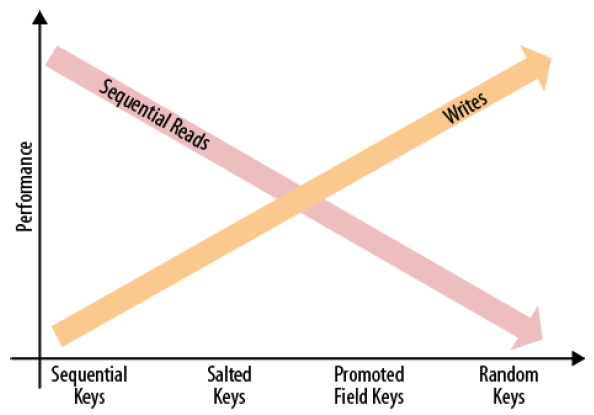
\includegraphics[width=0.46\linewidth]{images/timeseries.png}
			\end{figure}
	
\section{Apache Cassandra}
	\subsection{Overview}
	Cassandra is a distributed key-value that uses a column oriented model. There are no masters, every node can be whatever he wants, there is no single point of failure.\newline
	It has tunable consistency: it is often eventually consistent (AP) but it can shift to CP.\newline
	\newline
	It combines the HBase data model (one key per row, column and column families) and the Dynamo architecture (consistent hashing, anti-entropy replication and gossip-based membership).
	\subsection{Data Partitioning}
	The partitioning strategy can be changed on the fly but it needs to be chosen carefully because all data needs to be reshuffled.
		\subsubsection{Random Partitioner}
		It uses hash-based identifiers for keys and storage nodes (supports virtual nodes). Load monitoring (per ring) is added to consistent hashing: lightly loaded nodes are moved on the ring to alleviate heavily loaded ones. Deterministic choices are made about load balancing: divide the ring evenly with reference to the number of nodes.\newline
		Node addition and suppression requires re-balancing the cluster if there are no virtual nodes.
		\subsubsection{ByteOrdered Partitioner}
		It supports \textbf{range queries}, ensures row keys to be stored in sorted order. There is still a ring but keys are ordered lexicographically along the ring by their value. It might be bad for load balancing but range scan can be obtained by using column family indexes.
	\subsection{Data Replication}
	Replication is asynchronous, it walks down the ring, chooses \textit{N - 1} successor nodes as replicas and builds a preference list.\newline
	There are two main replication strategies, with \textbf{Simple strategy} the main replica is on the node responsible for a key and the additional ones are placed on the successor nodes. \textbf{NetworkTopology Strategy} allows better performance because of the knowledge of the datacenter layout (rack aware like HDFS). This requires Snitches  and optionally Zookeeper. Replica placement is independent in each datacenter.\newline
	There may be a potentially unbalanced load across the datacenter.
	\subsection{Data Model}
	The data model is column based. Each column stores counters containing timestamps. There could be expiring columns with a specified TTL. It also uses super columns to group multiple columns.
	\subsection{Read/Write Operations}
	Proxy nodes handle the interactions between the client and Cassandra, they determine the replicas for a given key and route the request to any replica.
		\subsubsection{Write request}
		The proxy node forwards the write request to all \textit{N} replicas but wait only for \textit{W} acks.\newline
		First the write is written in the \textbf{commit log}, then to an in-memory data structure (\textbf{memtable}) and finally writes are batched and periodically flushed to a persistent data structure: the \textbf{Sorted String Table}, SST (equivalent of HFile).\newline
		The memtables are organized in sorted order by row key and flushed to SSTables sequentially.\newline
		A single row can be stored in many SStables, at read time rows must be combined from all SSTables to produce the requested data.\newline
		To optimize this process \textbf{Bloom Filters} are used, they have \textit{k} hash functions hashing in the same \textit{m}-bit space. They are used when combining row data from multiple sources, they check if a requested row key exists in the SSTables before doing any disk seeks.
		\subsubsection{Read request}
		They use a similar mechanism to Dynamo if inconsistent replicas are detected, the number of replicas contacted upon a request depends on the consistency level.\newline
		When a node receives a read request, the row must be combined from all SSTables in that node and the data still stored in memtables.\newline
		To achieve higher performance Bloom Filters and the row level column index are used.
	\subsection{Consistency}
	Consistency is tunable and \textit{W} and \textit{R} are used as in Dynamo, but \textit{W + R $>$ N} is not mandatory.
		\subsubsection{Level ONE}
		\textit{W = 1}, one replica must write to commit log and memtable.\newline
		\textit{R = 1}, it returns a response from the closest replica (determined by the snitch).
		\subsubsection{Level QUORUM}
		\textit{W = floor(N/2 + 1)} and \textit{R = floor(N/2 + 1)}, it returns the record with the most recent timestamp.\newline
		If \textbf{LOCAL\_QUORUM}, it is restricted to a local data center.
		If \textbf{EACH\_QUORUM}, it must be satisfied across datacenters.
		\subsubsection{Level ALL}
		\textit{W = N} and \textit{R = N}.
		\subsubsection{Level ANY}
		Uses hinted handoff mechanism to add additional consistency for writes, it allows write to complete even if all \textit{N} replicas are down.
		\subsubsection{Level SERIAL}
		Lightweight transactions are used, they are a simple mechanism at the single key level, there is no support for multi-key transactions.
	
		
